\chapter{Results}
\label{chap:3}
\ChapterPageStuff{3}

\section{Introduction}
In \Cref{sec:ch2_preamble}, the methodology was created for a web-based software system. As described in this section, a user can have multiple systems and subsystems linked to their account. The implementation is done for multiple software systems in this section. The system implementation will focus more on the development of the logging mechanism, and the critical analysis will prioritise software maintenance using a utilisation analysis.

\section{Implementation}
In this section, the implementation of the development of the solution will be discussed using a test system to verify it. The test system is created in a \texttt{ASP.NET Core Web SDK} software environment.

\subsection{User activity types}
In \Cref{fig:ch2_user_based_actvity_classification} the user-based clarification flow diagram uses the \Cref{tbl:ch2_requirementsForUserActivtyEvent} to identify and capture some of the log attributes. The event logs should consist of multiple cases (\ref{fr:requirementsUserBased2}) that are the primary identifiers for the event log which is the user activity types.\par Using the basic operations of the system and what users interact with the user activate types can be made for each software system. For the test system, the basic use will be:

\begin{itemize}
	\item monitor resource usage dynamic dashboards,
	\item generate \texttt{PDF} reports of the displayed data.
\end{itemize}

Reporting and monitoring are important for this test system so the user activity types will need to focus on these activity types. To satisfy the \ref{fr:requirementsUserBased2}, \ref{fr:requirementsUserBased5} and \ref{fr:requirementsUserBased6} the user actvity types is defined in \Cref{tbl:ch3_testActivityTypes}.

\begin{table}[!htb]
	\centering
	\caption[Test user activity types]{\textit{Test user activity types}}
	\label{tbl:ch3_testActivityTypes}
	\begin{tabularx}{\textwidth}{|X|l|X|}
		\hline \textbf{Activity} & \textbf{Functional requirement} & \textbf{Description} \\
		\hline \texttt{SystemAccess} & \ref{fr:uatType1} & \RaggedRight This activity type detects when a user has navigated to a certain subsystem. \\ 
		\hline \texttt{General} & \ref{fr:uatType3} & \RaggedRight This general activity type is for all other activities that the user initiates that send \textit{HTTP request} back to the server. \\
		\hline \texttt{ReportExport} & \ref{fr:uatType3} & \RaggedRight The other main function of the system is for reporting purposes. Separating this type of activity in its category to capture all report generation activities that the user has initiated. \\ 
		\hline
	\end{tabularx}
\end{table}

\Cref{tbl:ch3_testActivityTypes} doesn't contain any session changes (\ref{fr:uatType3}) user types. These activities are only triggered when the user log's into their system or terminates their session by pressing the log-out button.

\subsection{Log attibutes}\label{sec:ch3_implementationLogAtrributes}
Using the functional requirements discussed in \Cref{sec:ch2_logAttributesRequirements} data columns are made for the user-based event's log attributes. These log attributes for a structured database are defined in \Cref{tbl:ch3_Log_Attributes}. 

\begin{table}[!htb]
	\centering
	\caption[Logging attributes]
	{\textit{Logging attributes}}
	\label{tbl:ch3_Log_Attributes}
	\begin{tabularx}{\textwidth}{|l|l|X|}
		\hline \textbf{Column name} & \textbf{Requirement ID} & \textbf{Description}\\
		\hline \texttt{ID} & \ref{fr:lpa1} & User based actvity primary identifier. \\
		\hline \texttt{TimeStamp} & \ref{fr:lpa2} & Date timesstamp when the activity has occur. \\
		\hline \texttt{ActivityType} & \ref{fr:lpa3} & Activity type of the log event. \\
		\hline \texttt{UserId} & \ref{fr:lpa4} & Identification number of the user associated with the log event. \\
		\hline \texttt{SystemId} & \ref{fr:lpa5} & System where the activity has occur. \\
		\hline \texttt{SubsystemId} & \ref{fr:lpa5} & Subsystem where the activity has occur. \\
		\hline \texttt{MetaData} & \ref{fr:lpa6} & Metadata captured from the \textit{HTTP request}. \\
		\hline \texttt{ClientId} & \ref{fr:lpa7} & Additional identifiers for the log event. In this case different configurations of the same system for a specific client. \\
		\hline
	\end{tabularx}
\end{table}

The data columns in \Cref{tbl:ch3_Log_Attributes} are used in a structured database. The test that is used is a \texttt{MySQL} database. This database has pre-existing tables that expand on other data such as the \texttt{UserId}, \texttt{SystemId} and \texttt{SubSystemId}. For the \texttt{MetaData} the \texttt{JSON} is similar to \Cref{fig:ch3_MetadataJson}.

\medskip

\begin{lstlisting}[style=json, caption={\textit{Metadata JSON}}, label={fig:ch3_MetadataJson}] 
	{
		"RequestOrigin": "/System/Subsystem1/GetData",
		"RequestElementID": "ButtonSaveCsv",
		"RequestParameters": {
			"tagIds": [
				"6284",
				"20320"
			],
			"toDate": "2020-04-06",
			"groupId": 2,
			"fromDate": "2020-03-30"
		}
	}
\end{lstlisting}

\clearpage

In \Cref{fig:ch3_MetadataJson} the main \texttt{JSON} parameters capture the following additional data for the user-based event:

\begin{itemize}
	\item \texttt{RequestOrigin} is the full file path of the subsystem that is being used and functions to fulfil the \textit{HTTP request}. Some of the subsystems consist of multiple individual files and this traces the origin of the \textit{HTTP request} function user-based activity accessed.
	\item \texttt{RequestElementID} is the last \textit{HTTP} element identification that the user interacted with that initiated the user-based activity.
	\item \texttt{RequestParameters} is the request parameters that are send with the \textit{HTTP request}. Any sensitive user data is either ignored by adding flags to certain subsystems or individual functions to not obtain the request's parameters.
\end{itemize}

\subsection{Logging points}
Table \ref{tbl:ch2_loggingPointRequirement} outlines the functional requirements for placing logging points in the software system. It's crucial to maintain consistency when capturing logs and placing them in a global location for all HTTP requests will ensure consistency. Filters can be used during the test system as it is a \texttt{ASP.NET Core Web SDK}. The filters can be initialised during the software system startup phase.\par For other web-based systems the central point where the \textit{HTTP requests} go through should be used to place single or multiple logging points. In other cases adding it for smaller groups of subsystems is also viable as long as the logs can be consistently captured when the requests come through. \par The filter of the test system is the primary component of the logging mechanism. It is responsible for capturing client-side log attributes and metadata using server-side parsing, as shown in Figure \ref{fig:ch2_loggingParse}. \par In \Cref{sec:ch3_implementationLogAtrributes} it has been discussed that some of the logs may contain sensitive data that should not be logged especially the metadata's request parameters. Adding a flag to indicate that certain subsystems' requests need to be ignored for the event logging should be added.\par This can also exclude certain parameters from being saved into the database. For the test system, it is an attribute added to certain controllers to ignore the obtained event logs and terminate the logging process.

\clearpage

\begin{figure}[!htb]
	\centering % cent the figure
	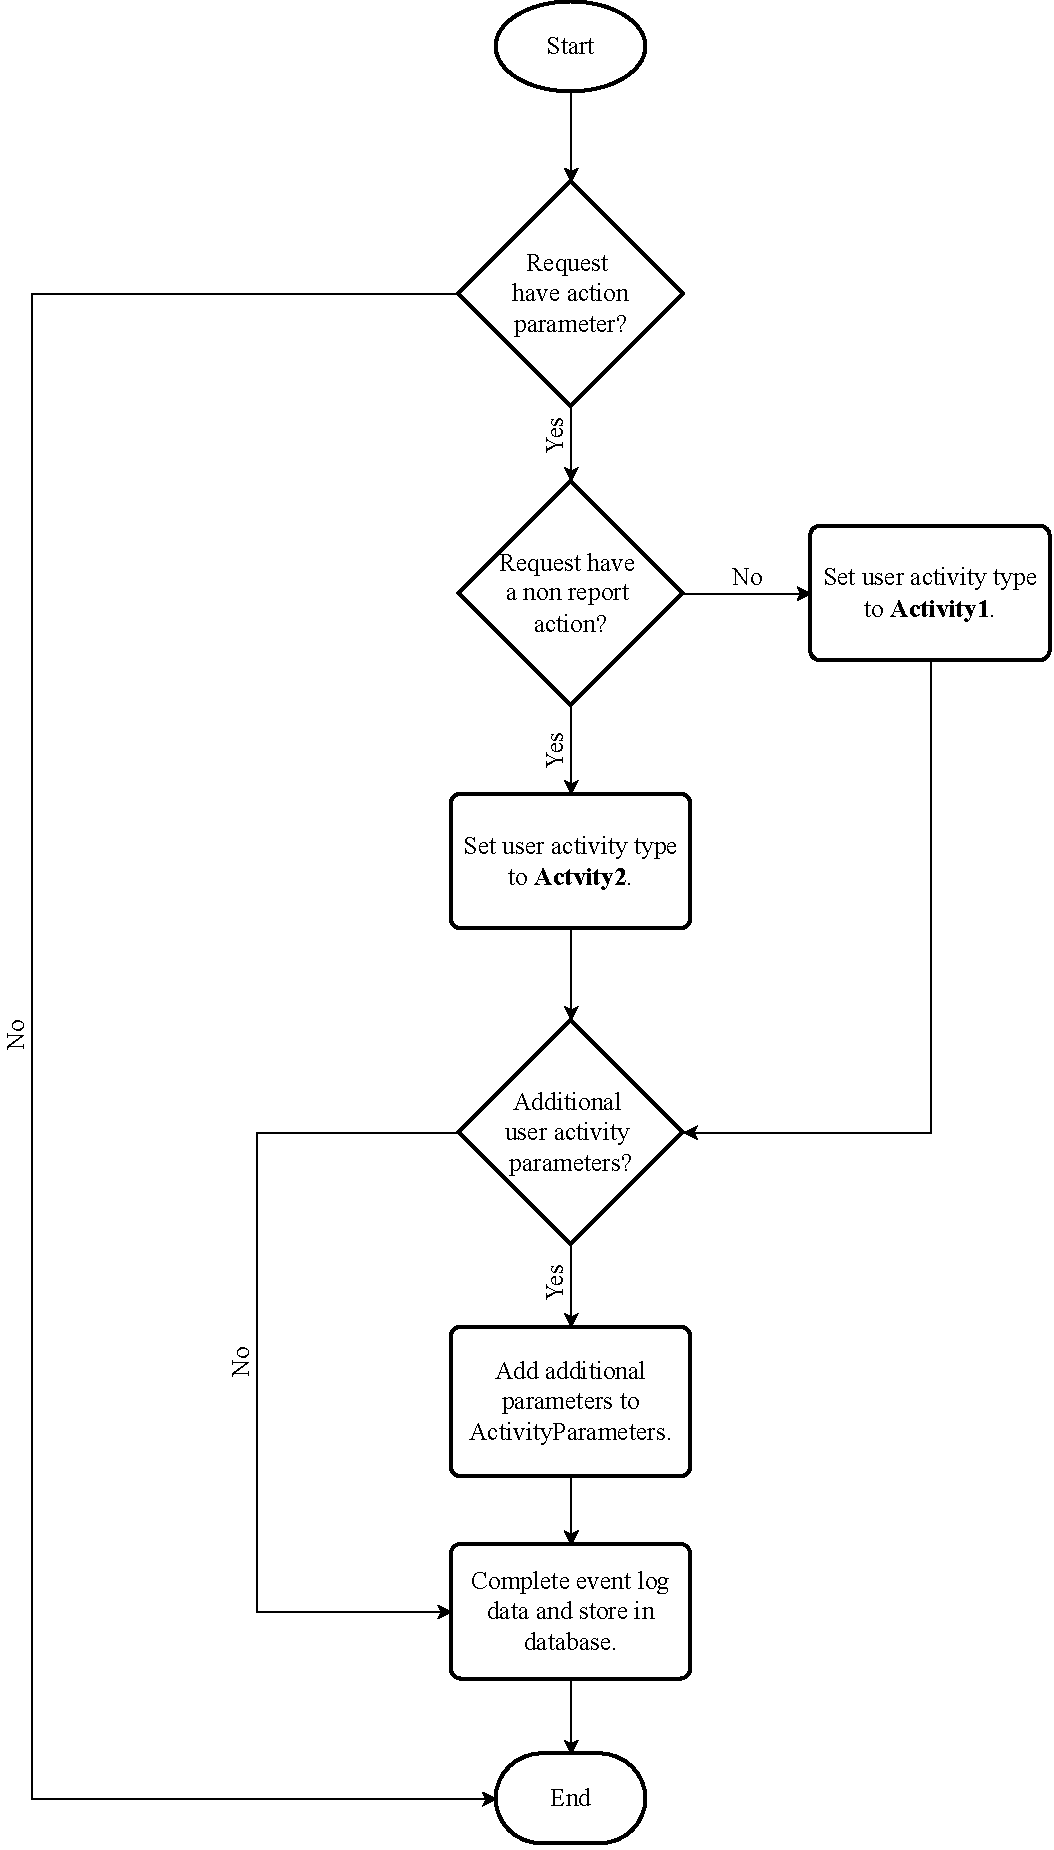
\includegraphics[width=0.75\textwidth]{Chapter2/DetailView_Flow/DetailView_Flow.pdf}
	\caption[User activity logging process]
	{\textit{User activity logging process}}\label{fig:ch3_loggingProcess}
\end{figure}

\clearpage

\subsubsection{Obtaining the element of user-based event}\label{sec:ch2_ElementObtaining}
In \Cref{sec:ch2_webApplicationArchitecture} the user-based activity event will be using a \textit{HTTP request} to send to the server when the user interacted with an \textit{HTML element}. For the functional requirements activity type (F/R 1.5.3) and metadata (F/R 1.5.6) in \Cref{tbl:ch2_keyLoggingAttributes} the \textit{HTML element} needs to be obtained to get the element's tag and identification text.\par This can be difficult to obtain due to \textit{bubbling}\footnote{\textbf{Bubbling} is when an event happens on an element, it first runs the handlers on it, then on its parent, then up on other ancestors. \cite{EventBubbling}.} that may occur when searching for the element that the user specifically interacted with. \Cref{fig:ch2_event_bubbling} is the event bubbling propagation.

\begin{figure}[!htb]
	\centering % cent the figure
	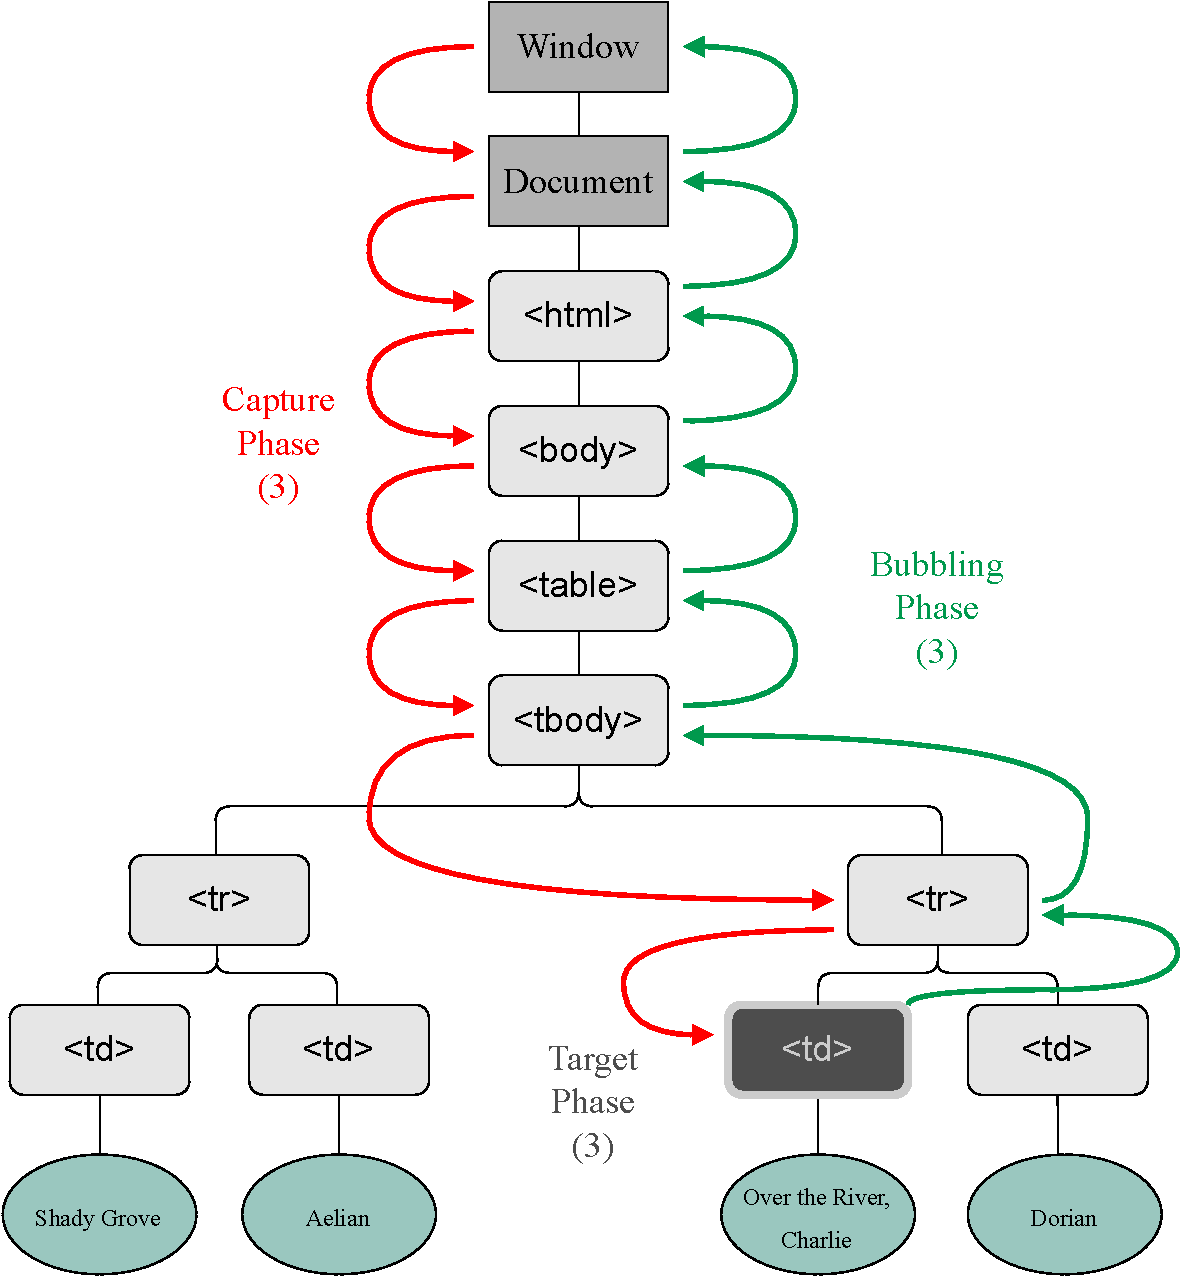
\includegraphics[width=0.8\textwidth]{Chapter2/event_bubbling/event_bubbling.pdf}
	\caption[JavaScript event propagation]
	{\textit{JavaScript event propagation~\cite{EventBubbling}}}\label{fig:ch2_event_bubbling}
\end{figure}

In \Cref{fig:ch2_event_bubbling} is the event propagation example of a child element that has been clicked on which executes a DOM event. The event propagation consists of three phases~\cite{EventBubbling}:

\begin{itemize}
	\item \textit{Capturing phase:} The event propagates downwards to the targeted element that the user interacted with.
	\item \textit{Target phase:} The event reaches the targeted element to execute the DOM event.
	\item \textit{Bubbling phase:} The event bubbles up from the targeted element
\end{itemize}

Capturing the targeted element may be difficult as some web pages may have more complex HTML, which can cause event propagation to fail to obtain the correct element information that the user interacted with. In such cases, it is more accurate to obtain the targeted element by identifying the last known element that the user hovered over on the user interface, as another DOM event may have started during the initial element's event.\par \Cref{fig:ch2_element_event_capturing} shows the flow diagram to capture the element that the user interacted with for the user-based activity log. This code segment will be initiated during the \texttt{beforeSend} operation of the \textit{AJAX request} to filter HTML elements by predefined allowed elements. Filtering the element tag names ensures that unwanted, more complex elements or basic elements that are not expected to be the initiator of the event, will be excluded. 

\begin{figure}[!htb]
	\centering % cent the figure
	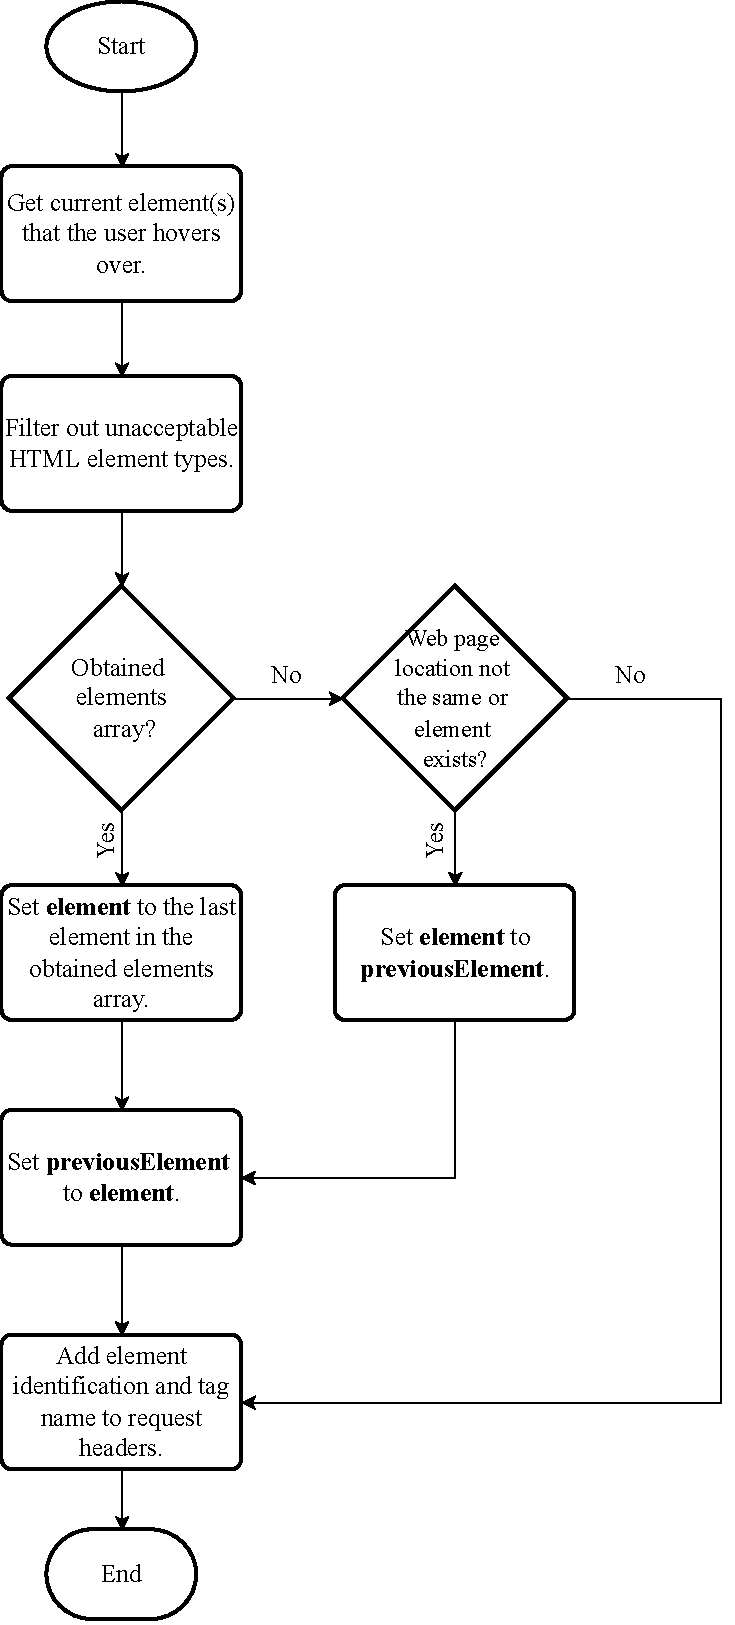
\includegraphics[width=0.55\textwidth]{Chapter2/element_capturing/element_capturing.pdf}
	\caption[HTML element capturing flow diagram]
	{\textit{HTML element capturing flow diagram}}\label{fig:ch2_element_event_capturing}
\end{figure}

If the web location has already changed or no element exists, the contents of the page may have already changed during the event propagation. Therefore, the last known element that the user hovered over must be used, as it is most likely to be the element that the user interacted with. This approach ensures that there is always an element that has been detected and parsed with the request header in most UI changes.

\clearpage

\subsection{Log analysis}\label{sec:ch3_implementationLogAnalysis}
In \Cref{ch2:sec_system_utilisation_analysis}, the functional requirements for log analysis are defined. For this implementation of log analysis, a custom log analysis tool is created to:

\begin{itemize}
\item Visually present user-based event logs through the log analysis tool as required in \Cref{tbl:ch2_logAnalysisToolFR}.
\item Filter user-based event logs through different criteria described in \Cref{tbl:ch2_utilisationCategories}.
\item Analyse logs for maintenance prioritisation as shown in \Cref{tbl:ch2_maintenancePriortising}.
\end{itemize}

\section{Verification}
The log analysis tool will be used to verify the implementation of the logging mechanism on the test system. This system is created in a \texttt{.NET Framework} software environment and uses a \texttt{MySQL} database to store the logging events.

\subsection{Log attributes}
The captured log attributes of \Cref{tbl:ch3_Log_Attributes} that are captured by the logging points are shown in \Cref{fig:ch3_UAT_menu}.

\begin{figure}[!htb]
	\centering % cent the figure
	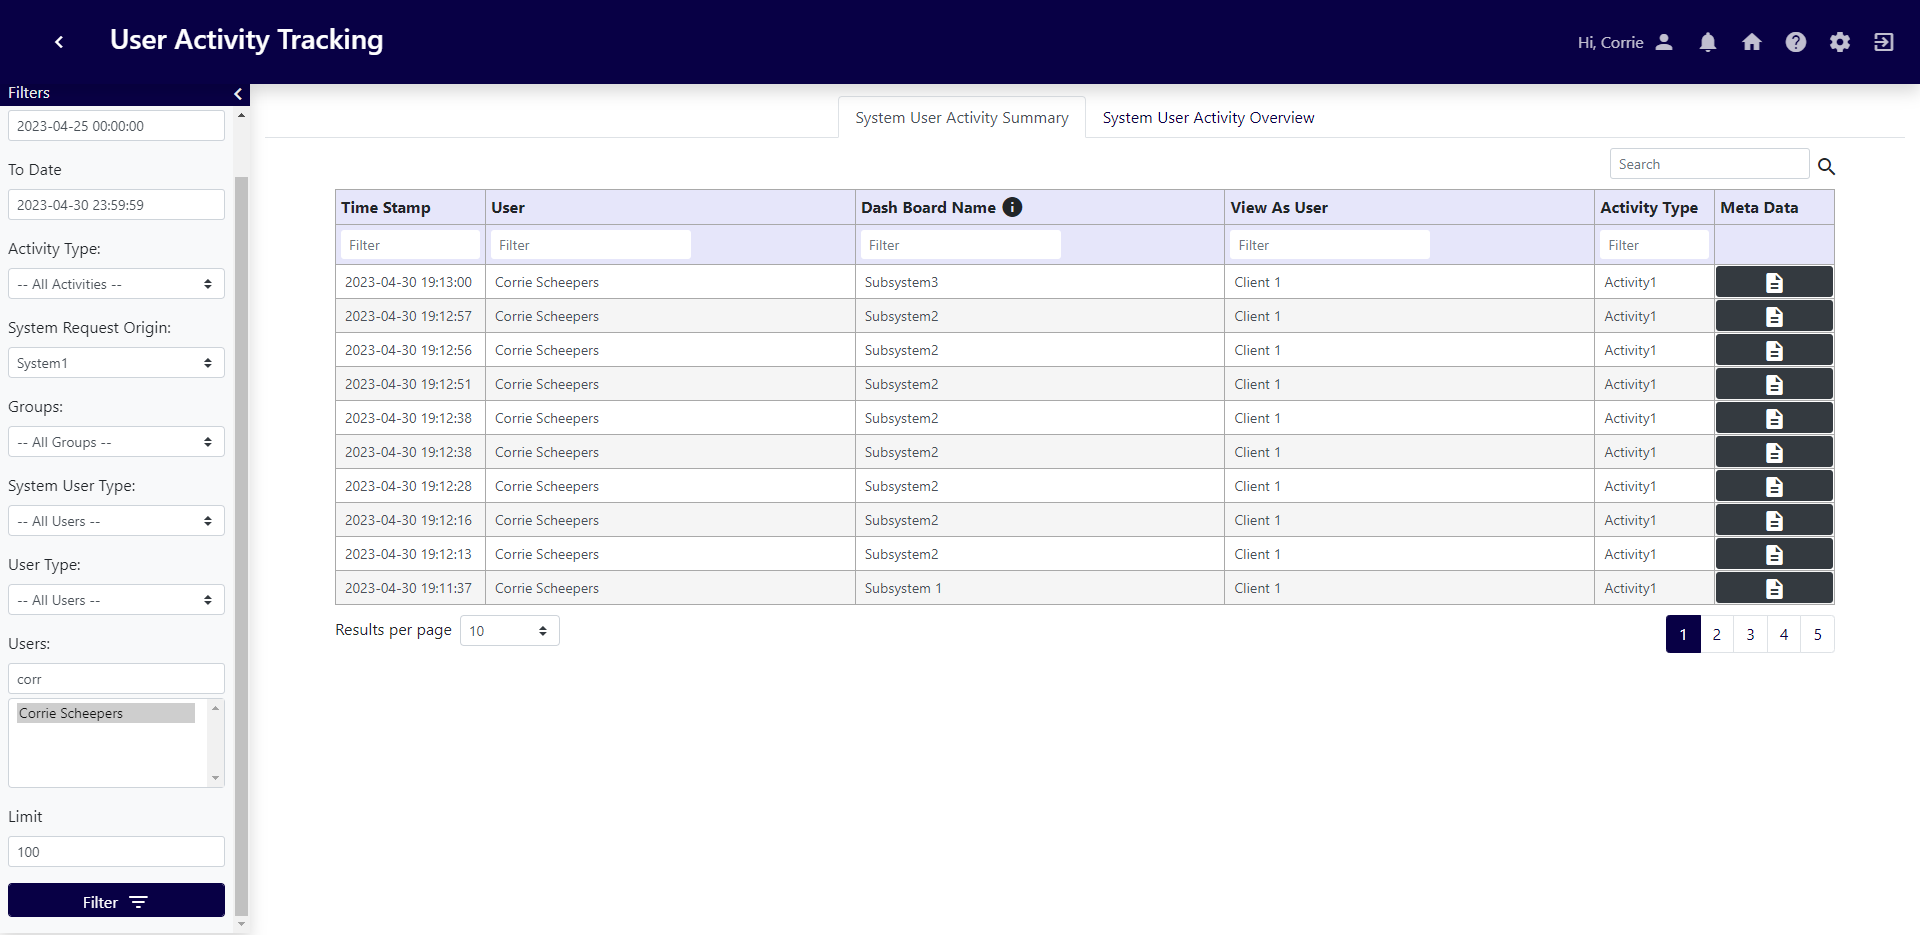
\includegraphics[width=0.99\linewidth]{img/ch3/analysis/UAT_menu.png}
	\caption[Interactive user activity viewer]
	{\textit{Interactive user activity viewer}}\label{fig:ch3_UAT_menu}
\end{figure}

\Cref{fig:ch3_UAT_menu} confirms that the required log attributes defined in \Cref{tbl:ch3_Log_Attributes} are being tracked for the test systems. The user interface created to display the logs is designed to be more understandable for users who analyze the logs. The meta-data is displayed in a \texttt{JSON} format as in \Cref{fig:ch3_JSON_Test_Result}.

\clearpage

\begin{figure}[!htb]
	\centering % cent the figure
	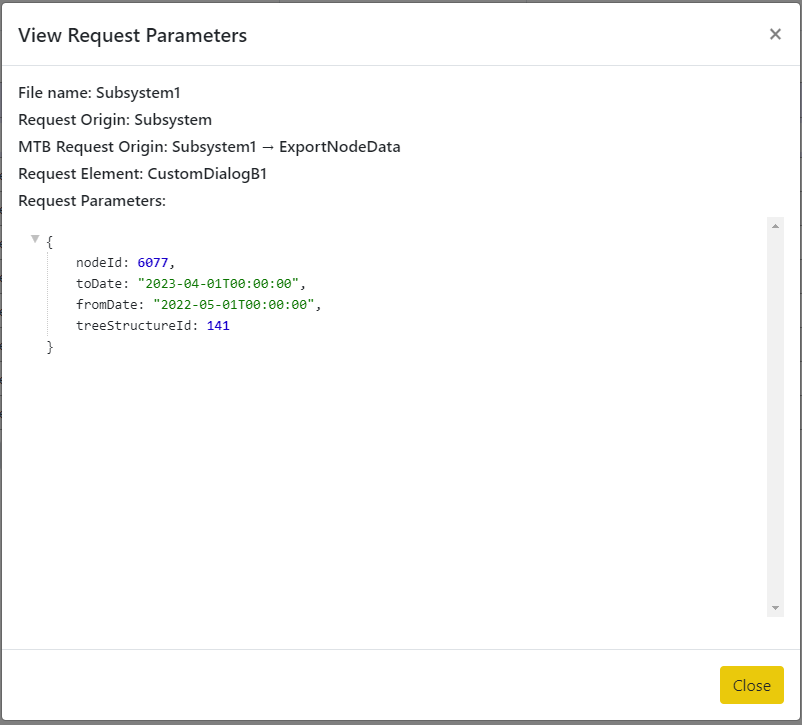
\includegraphics[width=0.65\linewidth]{img/ch3/analysis/UAT_request_params.png}
	\caption[JSON test request parameter data]
	{\textit{JSON test request parameter data}}\label{fig:ch3_JSON_Test_Result}
\end{figure}

\Cref{fig:ch3_JSON_Test_Result} includes additional parameters described in \Cref{fig:ch3_MetadataJson}. The \texttt{RequestElementID} is obtained using the element capturing method described in \Cref{fig:ch2_element_event_capturing}, while the other metadata parameters are captured using the built-in methods available in \texttt{C\#}.

\subsection{Log analysis}
The log analysis of the obtained logs shown in \Cref{fig:ch3_UAT_menu} is done in the same interactive dashboard. \Cref{fig:ch3_UAT_menuAnalysis} is a comparison of the obtained logs for the subsystems.

\begin{figure}[!htb]
	\centering % cent the figure
	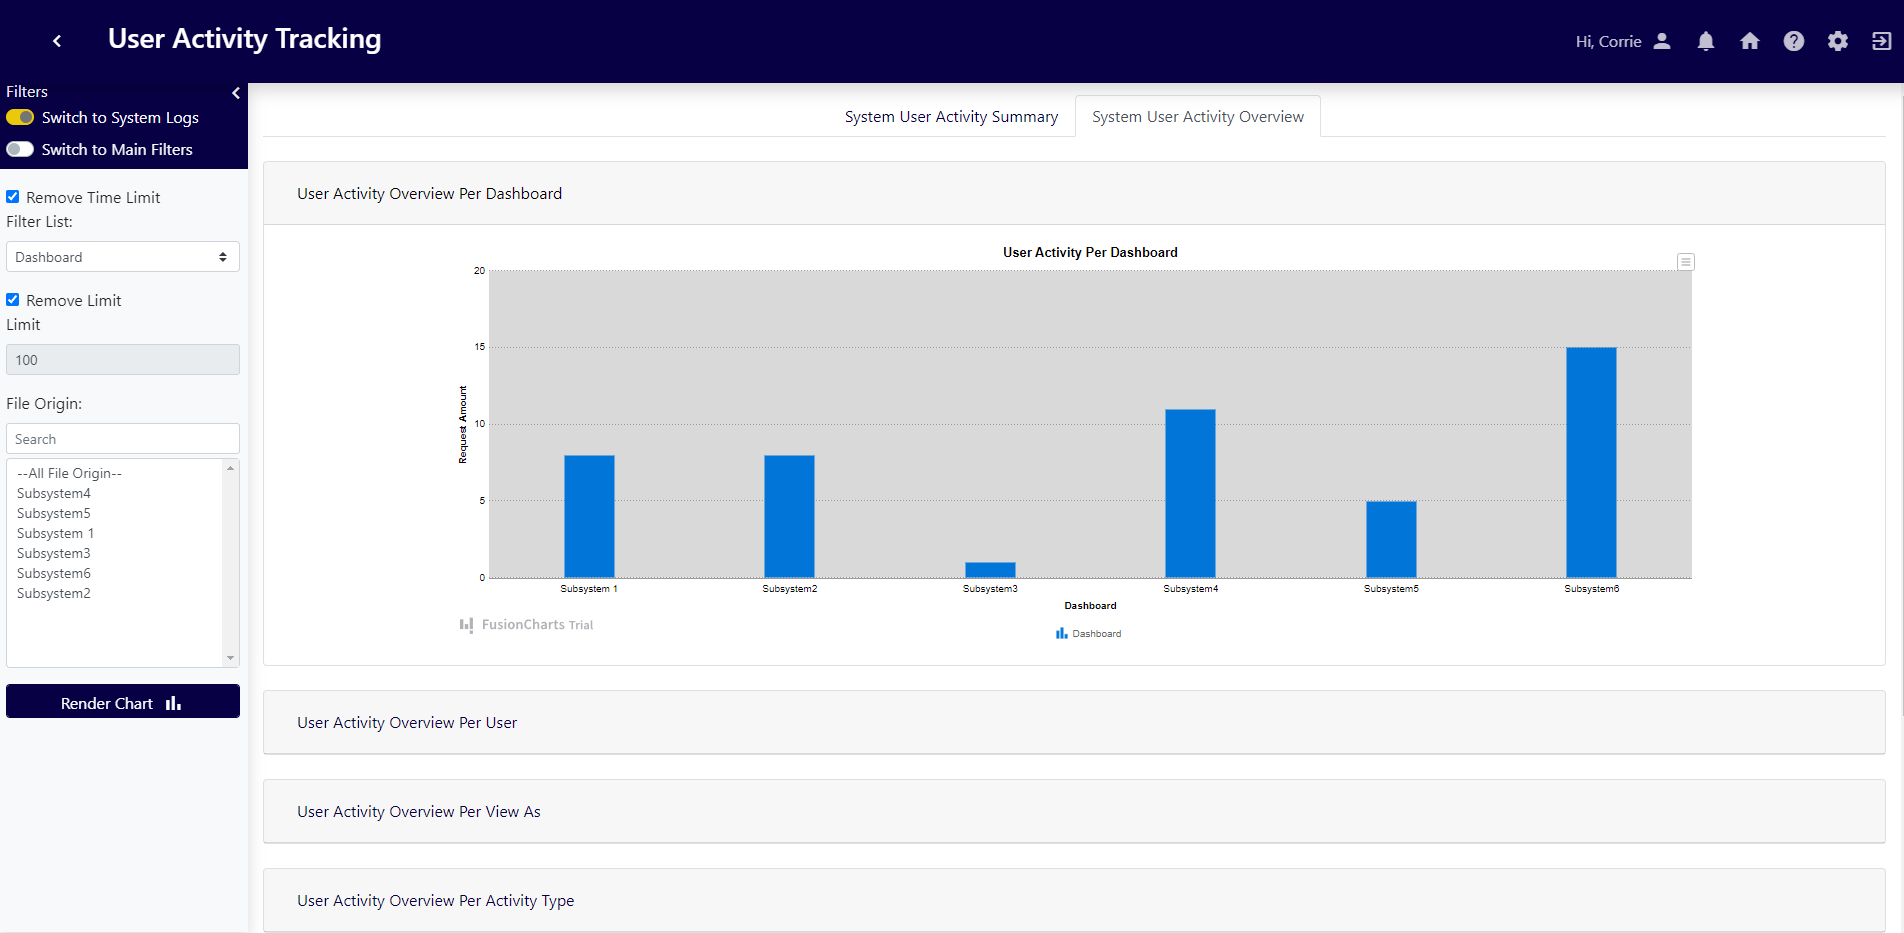
\includegraphics[width=0.99\linewidth]{img/ch3/analysis/UAT_menu_analysis.png}
	\caption[Interactive user activity viewer]
	{\textit{Interactive user activity viewer}}\label{fig:ch3_UAT_menuAnalysis}
\end{figure}

\clearpage

\Cref{tbl:ch2_utilisationCategories} provides the functional requirements for various utilization categories. By comparing these categories to each other in the obtained user logs, different categories can be compared, as shown in \Cref{fig:ch3_UAT_menuAnalysis}. Furthermore, \Cref{fig:ch3_UAT_menuActivities} compares different types of user activities.

\begin{figure}[!htb]
	\centering % cent the figure
	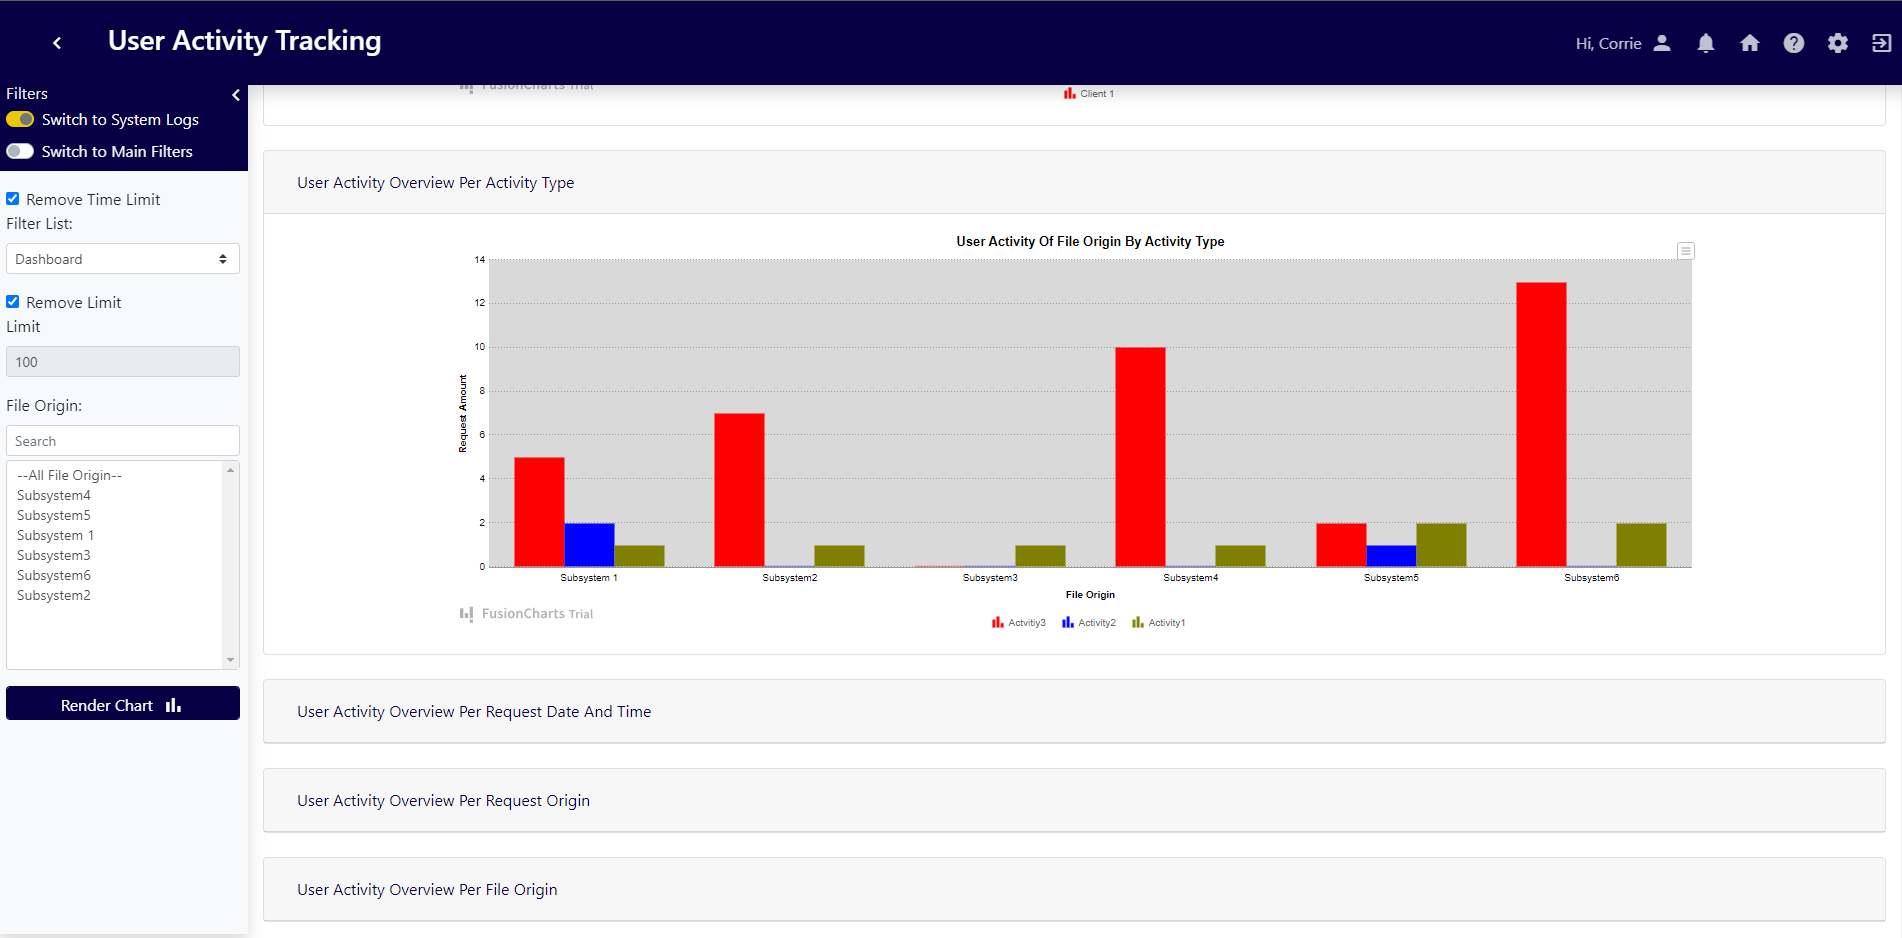
\includegraphics[width=0.99\linewidth]{img/ch3/analysis/UAT_menu_activities.png}
	\caption[Interactive user activity log analysis]
	{\textit{Interactive user activity log analysis}}\label{fig:ch3_UAT_menuActivities}
\end{figure}

\subsection{Maintenance priortising}
For the test system, maintenance prioritisation recommendations can be made as described in \Cref{sec:ch2_utilisationImprovements}. A rating system can be used to rank the most critical software systems that need to be prioritised, which can aid in software maintenance efforts.\par Using \Cref{eq:ch2_maintenanceFactorSimplified} the maintenance priority factor $M_{PF}$ can be determined for a set of systems {$S1,~S_2,~...,~S_N$} which has captured user activities per system $A_X$. The system will also have several users linked to each system $P_X$. These parameters are set for the test system as in \Cref{tbl:ch3_testData}.

\begin{table}[!htb]
	\centering
	\caption[Data for validating test system]
	{\textit{Data for validating test system}}
	\label{tbl:ch3_testData}
	\begin{tabularx}{\textwidth}{|X|X|X|}
		\hline \textbf{System ($S_X$)} & \textbf{Users per system ($P_X$)} & \textbf{Number of events ($A_X$)} \\
		\hline $S_1$ & 226 & 11 \\
		\hline $S_2$ & 269 & 5 \\
		\hline $S_3$ & 156 & 8 \\
		\hline $S_4$ & 155 & 1 \\
		\hline $S_5$ & 145 & 13 \\
		\hline $S_6$ & 154 & 8 \\
		\hline
	\end{tabularx}
\end{table}

The activities in \Cref{tbl:ch3_testData} were generated by a single user who navigated through and interacted with the system, as shown in \Cref{fig:ch3_UAT_menuActivities,fig:ch3_UAT_menuAnalysis}. To compare the effect of the total number of user activities per system, we focus on $S_3$ to $S_6$, which have similar numbers of active users who can access the system. For the test system $S$, it is expected that $S_1$ will have the highest maintenance priority factor, given that it has:

\begin{itemize}
	\item The second highest number of users linked to it. This should increase its normalised active user factor.
	\item It has the second-highest number of observed user events that were captured.
\end{itemize}

$S_4$ has the least total number of user events but has about the same number of users linked to it. This should have the lowest maintenance factor as a lower number of activities will indicate that the system is not used as much as systems like $S_3$ and $S_6$. These other two systems have higher captured user events.\par Using \Cref{eq:ch2_priorityNormalised} to calculate each subsystem's normalised priority factor using the number of users that have access to the system; also using \Cref{eq:ch2_eventNormalised} to calculate the normalised activities, the results are shown in \Cref{tbl:apx_testB_Normilised}.


    \begin{xltabular}{\textwidth}{|X|X|X|X|X|X|X|}
        \caption[Test data]
        {\textit{Test data}}
        \label{tbl:apx_testB_Normilised} \\
        
        \hline
        \textbf{$S_{X}$} & \textbf{$P_X$} & \textbf{$P_N$}  & \textbf{$A_X$} & \textbf{$A_N$} & \textbf{$M_{PF}$} & \textbf{$P_{R}$} \\
        \hline
        \endfirsthead

        \multicolumn{7}{c}
        {\tablename\ \thetable{} -- continued from previous page} \\
        \hline
        \textbf{$S_{X}$} & \textbf{$P_X$} & \textbf{$P_N$}  & \textbf{$A_X$} & \textbf{$A_N$} & \textbf{$M_{PF}$} & \textbf{$P_{R}$} \\ 
        \endhead

        \multicolumn{7}{|r|}{{Continued on next page}} \\ \hline
        \endfoot

        \hline
        \endlastfoot
    $S_1$ & 226 & 0.6504 & 11 & 0.8333 & 0.5420 & 1 \\ \hline
 $S_2$ & 269 & 1.0000 & 5 & 0.3333 & 0.3333 & 2 \\ \hline
 $S_3$ & 156 & 0.0813 & 8 & 0.5833 & 0.0474 & 3 \\ \hline
 $S_6$ & 154 & 0.0650 & 8 & 0.5833 & 0.0379 & 4 \\ \hline
 $S_4$ & 155 & 0.0732 & 1 & 0.0000 & 0.0000 & 5 \\ \hline
 $S_5$ & 146 & 0.0000 & 13 & 1.0000 & 0.0000 & 5 \\ \hline
    \end{xltabular}
    

In \Cref{tbl:apx_testB_Normilised}, $P_N$ for $S_1$ and $S_2$ is the highest, as most users have access to them. Additionally, $S_1$ and $S_5$ have the highest $A_N$ rating, indicating that they were the most used systems. As previously stated, it is expected that $S_1$ will require the most maintenance activities. The systems with lower maintenance activities and still have similar active users linked to them have a lower maintenance priority factor.

\section{Case studies}

\subsection{Case study identification}

\subsection{Case study results}

\subsubsection{System A results}

\begin{landscape}
	\begin{figure}[!htb]
		\centering % cent the figure
		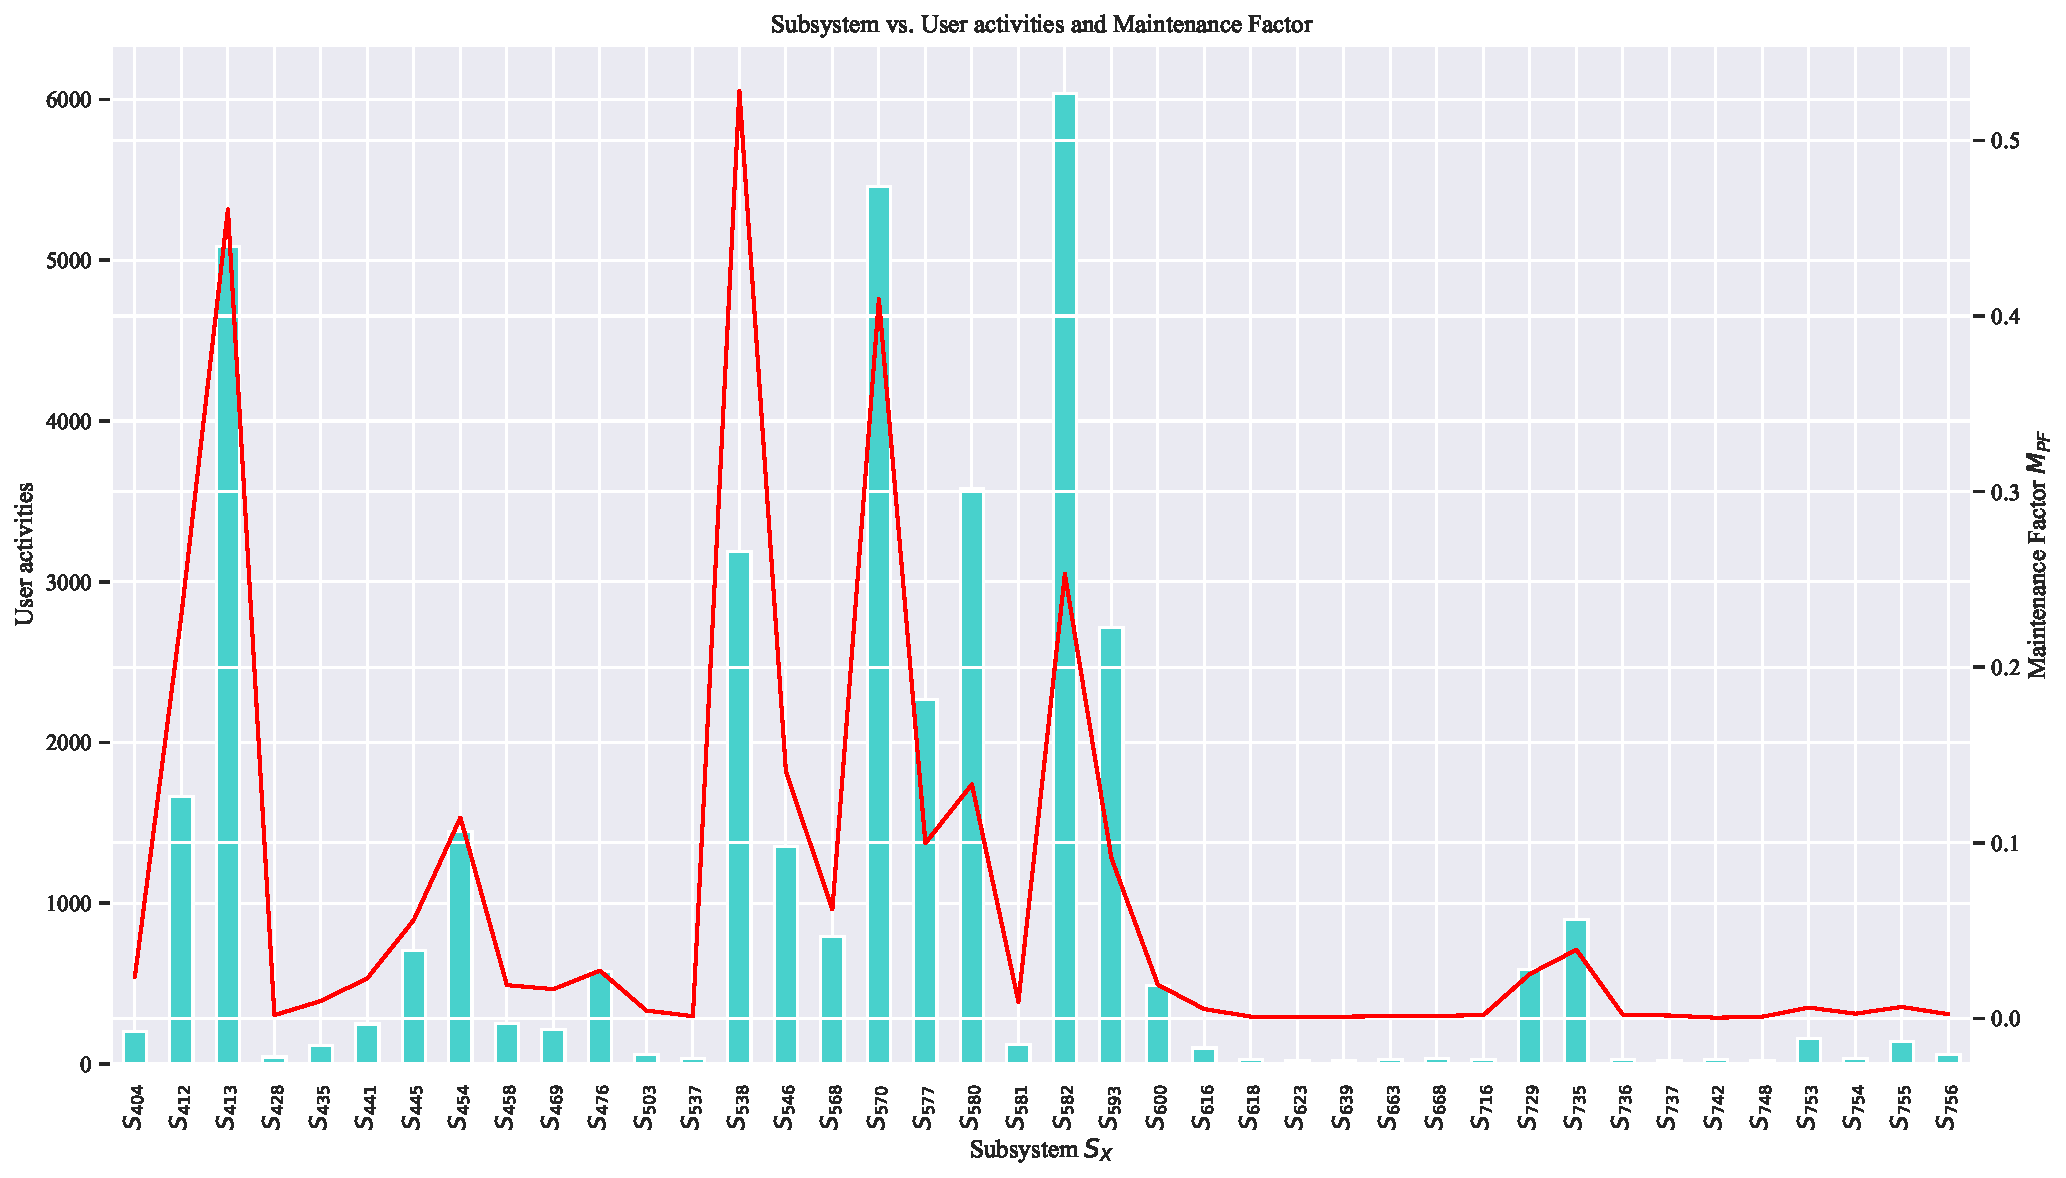
\includegraphics[width=0.95\linewidth]{img/ch3/analysis/case_A_subsystems_1.pdf}
		\caption[Case study 1 subsystem activities part 1]
		{\textit{Case study 1 subsystem activities part 1}}\label{fig:ch3_saS1S246}
	\end{figure} 
\end{landscape}

\subsubsection{System B results}

\begin{landscape}
	\begin{figure}[!htb]
		\centering % cent the figure
		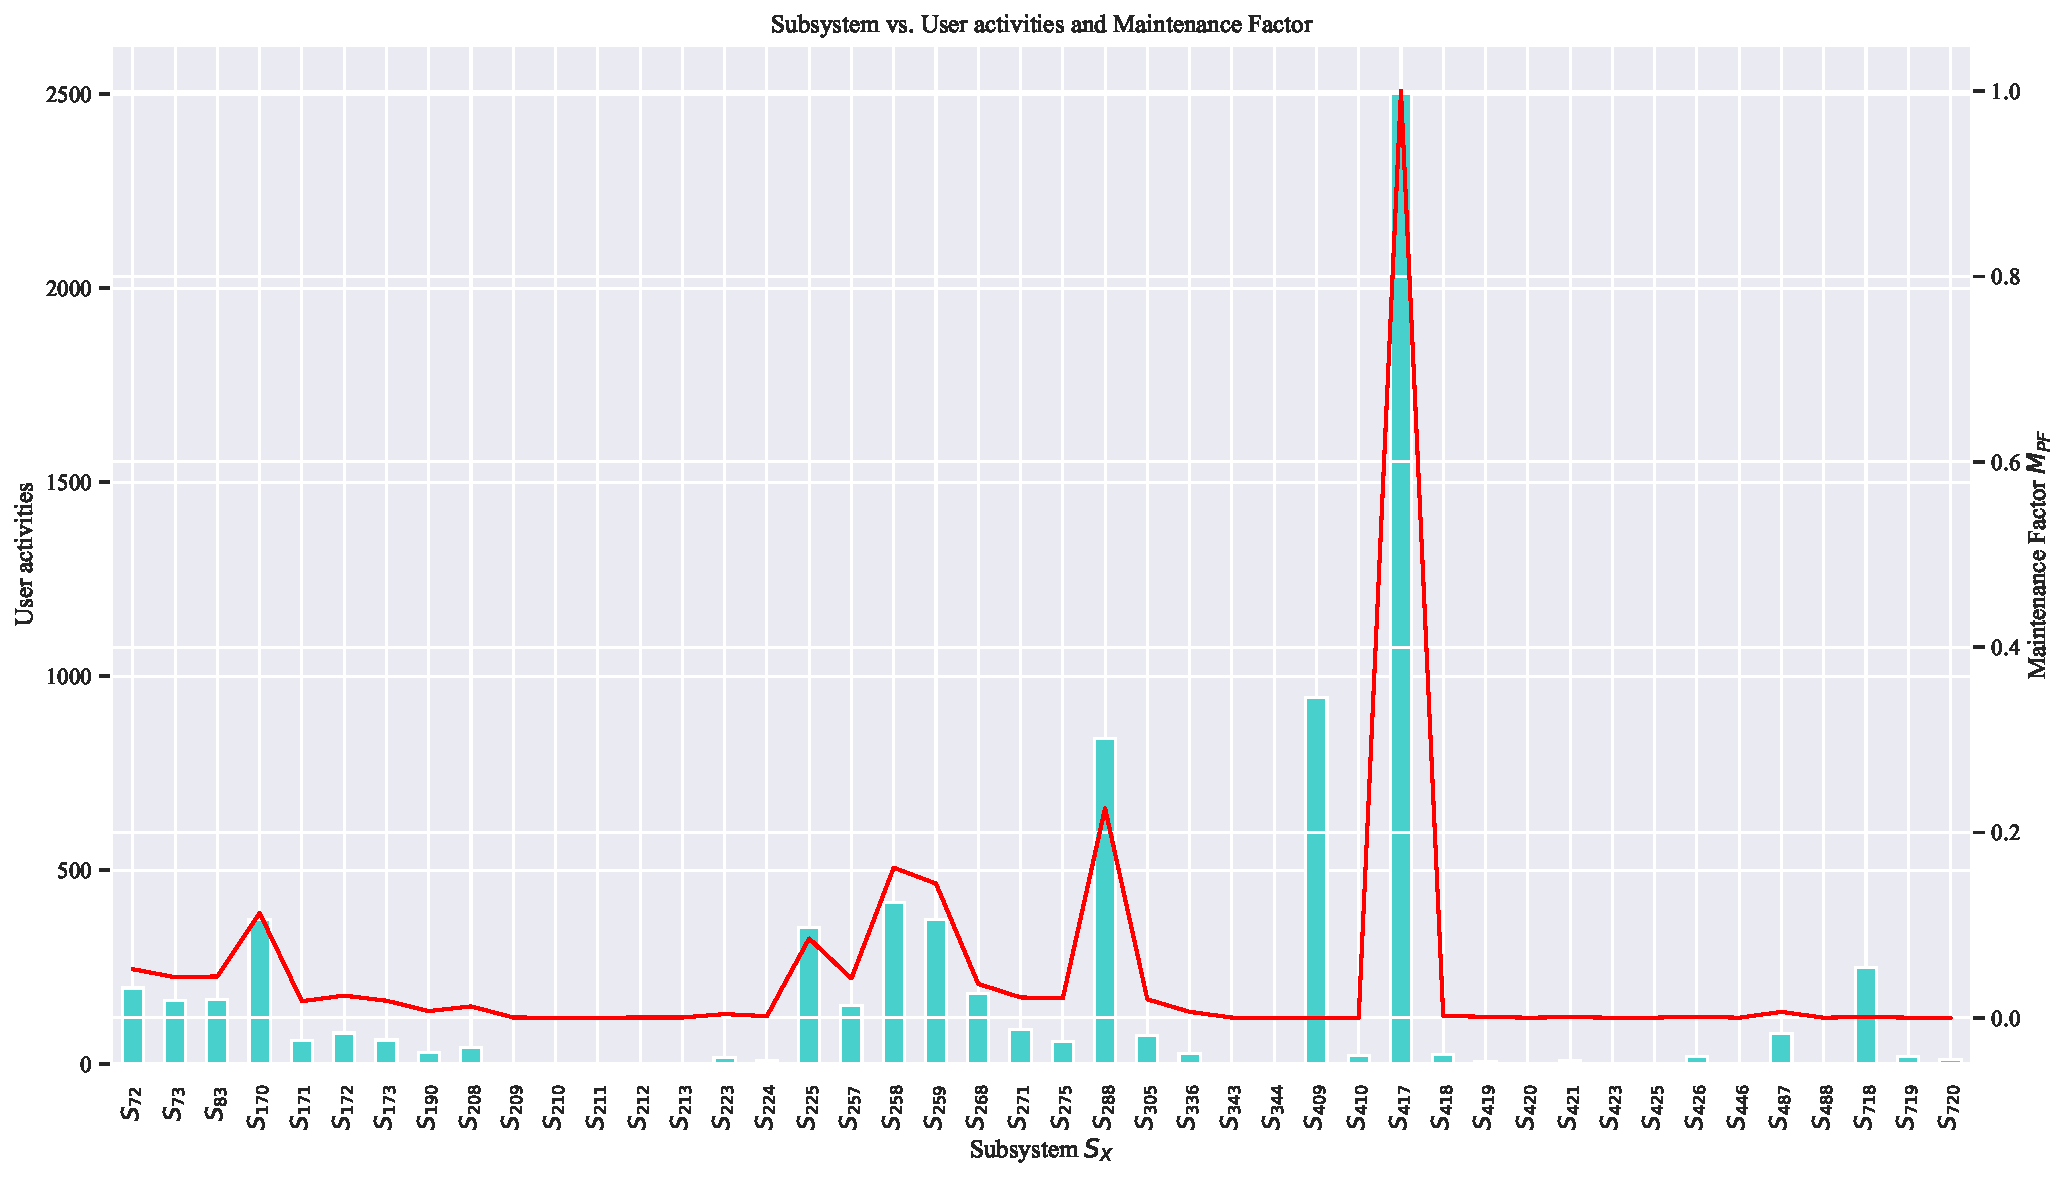
\includegraphics[width=0.95\linewidth]{img/ch3/analysis/case_B_subsystems_1.pdf}
		\caption[Case study 2 subsystem activities part 1]
		{\textit{Case study 2 subsystem activities part 1}}\label{fig:ch3_sbS1S246}
	\end{figure} 
\end{landscape}

\clearpage

\subsection{Critical analysis results}

\section{Conclusion}